\section{Анализ предметной области}
\subsection{Характеристика СКУД и её назначение}

Сегодня под термином СКУД (Система контроля и управления доступом) понимается вид физической безопасности, который управляет точками входа в ваш бизнес или внутренние помещения здания. Простой пример СКУД -- ворота, физически не допускающие неавторизованных пользователей и позволяющие войти только авторизованным пользователям.

Минимальная функциональность СКУД – проверка наличия кода в базе данных и, при положительном результате, выполнение разблокировки преграждающего устройства. Однако в настоящее время существует некий «джентльменский набор» выполняемых действий, которые должны быть реализованы в любой уважающей себя СКУД – это контроль кого, куда и когда пускать.

В некоторых случаях к этому набору добавляются функции запрета повторного прохода (запрет на повторный вход, если не было выхода) и запрет прохода во внутренние помещения без пересечения проходной (внешнего периметра).

В большинстве случаев профессиональные СКУД обеспечивают и иные режимы проходов, например, проход по двум ключам,  шлюз, контрольный обход территории, дисциплина проходов во внутренние зоны.

Три лидера отрасли в РФ, каждый из которых разработал инновационные системы контроля доступа -- <<АAМ Системз>>, <<Равелин>> и <<PERCo>> разрабатывают передовые системы безопасности, которые являются универсальными, масштабируемыми и гибкими, оставаясь при этом высокофункциональными.
%Актуальность данной темы заключается в необходимости установки порядка и правил на объекте с большим количеством людей, минимизации влияния ручного управления на систему, а также сокращении расходов на персонал, занимающий потенциальные места для продажи.

\subsection{Ключевые элементы системы контроля доступа и принцип их работы}
\subsubsection{Учётные данные}

Учетные данные контроля доступа используют RFID (радиочастотную идентификацию) для передачи сигналов на панель контроля доступа. Каждая метка имеет уникальный зашифрованный идентификационный номер. Владелец системы может выдать всем сотрудникам метки одного типа, но при этом настроить одну метку на разрешение входа, а другую - на запрет входа в определенные зоны здания.

УД бывают следующих видов:

\begin{itemize}
	\item пароль или пин-код;
	\item биометрия.
\end{itemize}


\paragraph{Пароль или ПИН-код}

Преимущество парольных систем по сравнению с системами дискреционного контроля доступа на основе матрицы доступа заключается в том, что в них нет объекта, связанного с монитором безопасности, который хранит информацию о контроле доступа к конкретным объектам. Кроме того, парольные системы обеспечивают безопасность даже в том случае, если посторонние лица имеют неограниченный или технически возможный доступ к носителям, на которых записаны и хранятся зашифрованные объекты. Эти преимущества парольных систем управления доступом делают их чрезвычайно распространенными в документальных информационных системах.

\paragraph{Биометрия}

Объекты со строгими требованиями к соблюдению норм и правил, такие как больницы и производственные предприятия, требуют особенно надежных систем контроля доступа и безопасности. Биометрические технологии используют измерения тела и физические характеристики для поиска уникальных идентификационных признаков человека (обычно отпечатков пальцев, сканирования сетчатки глаза или лица), чтобы сделать идентификацию положительной. 

\subsubsection{Устройства-носители данных}

Такие устройства выполняют идентичные функции, выступая носителями данных вместо пользователя.

Самыми распространёнными устройствами такого вида являются:

\begin{itemize}
	\item данные устройства;
	\item брелок или карта доступа.
\end{itemize}

\paragraph{Данные устройства}

Для контроля доступа с помощью мобильных устройств используются смартфоны, планшеты и носимые электронные устройства, которые служат удостоверением личности пользователя для входа в офис или другие деловые помещения. Поскольку большинство работодателей поощряют тенденцию Bring Your Own Device (BYOD), контроль доступа с помощью приложений стал одним из самых эффективных инструментов для обеспечения дополнительного уровня безопасности в любой организации. В настоящее время электронные устройства позволяют осуществлять биометрическую аутентификацию без необходимости инвестировать в дорогостоящие биометрические считыватели.

\paragraph{Брелок или карта доступа}

Карта доступа – это идентификатор пользователя, на котором содержится некая информация – ключ, открывающий дверь или доступ к ресурсам. 
Системы контроля доступа на основе карт играют важную роль в защите вашей собственности. Системы доступа без ключа - это эффективный и доступный способ обеспечить безопасность людей, помещений и данных. Карточные системы подходят для объектов любого типа - охраняемого склада, общежития или коммерческого здания.

\subsubsection{Устройство СКУД}

Базовая современная СКУД состоит из:

\begin{itemize}
	\item считывателя;
	\item контроллера;
	\item замка.
\end{itemize}

\paragraph {Считыватель}

Считыватель меток находится на одной или обеих сторонах двери - на одной стороне двери, если система контролирует только вход, или на обеих сторонах, если система контроля доступа контролирует вход и выход. Считыватель содержит антенну, которая подключается к панели контроля доступа и получает от нее питание.
Когда человек входит в здание со своей меткой контроля доступа, на антенну считывателя поступает его зашифрованный идентификационный номер.

\paragraph {Контроллер}

Контроллер - это ядро системы. В нем хранится информация об авторизации, которая настраивается администратором системы. Контроллер получает зашифрованный номер метки от считывателя, расшифровывает его, затем сравнивает ID-номер с ID-номерами, которые были загружены в систему. Если номера совпадают, и пользователь имеет право доступа к двери, дверь разблокируется.

\paragraph {Замок}

Панель управления доступом, или контроллер, управляет электрическим замком двери. Если пользователю разрешено войти в здание, дверь автоматически разблокируется и может быть открыта.
Общая схема устройства системы изображена на рисунке ~\ref{fig:commonscheme1}.
\begin{figure}
	\centering
	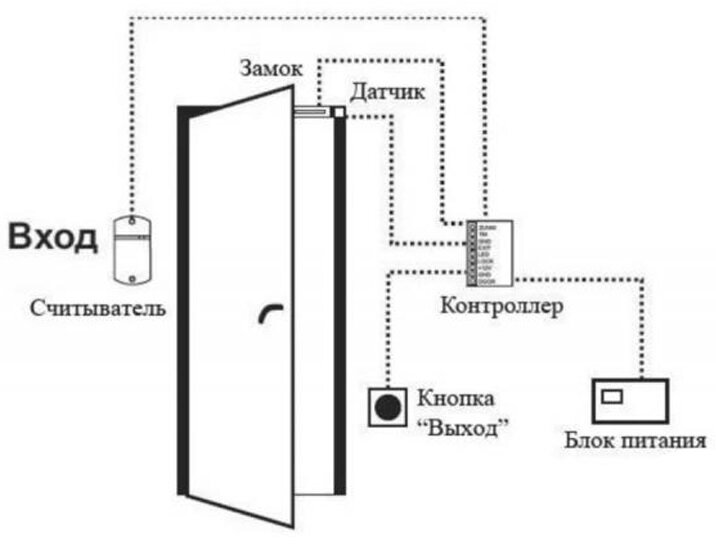
\includegraphics[width=0.7\linewidth]{images/CommonScheme1}
	\caption{Схема устройства современной СКУД}
	\label{fig:commonscheme1}
\end{figure}

\subsection{Анализ категорий пользователей СКУД}

Система контроля и управления доступом - неотъемлемая часть безопасности. Она обеспечивает дополнительный уровень защиты, позволяя контролировать и отслеживать тех, кто имеет доступ к объекту защиты.

СКУД применима в отраслях - в здравоохранении, корпоративном, образовательном и государственном секторах. Сегодня они применяются на различных объектах, таких как стационарные, долговременные и жилые учреждения, больницы, муниципалитеты, кондоминиумы, распределительные комплексы, малые и крупные предприятия, а также колледжи и университеты.

Среди пользователей программного обеспечения СКУД -- системные администраторы и специалисты по информационной безопасности, нанятые организацией с целью контроля правил системы, устранения неполадок, проведения аудитов безопасности, поддержания работоспособности, внесения изменений.

В нашем случае, на круизном лайнере, пользователем приложения является человек из экипажа, занимающийся внесением данных пассажиров в базу, наложением штрафов, созданием правил для входа в те или иные сектора, манипуляцией дверьми во время ЧС и т.д.

\subsection{Перспективы развития}
В перспективе развития СКУД на круизном лайнере ключевым является масштабирование её возможностей. Для самой системы это может быть увеличение быстродействия, расширение набора правил и ограничений, добавление умных систем обнаружения (камер) для фиксации нарушений и автоматического наложения штрафов, внедрение технической поддержки в реальном времени для нерядовых случаев.

В перспективе развития ПО для СКУД, ключевым является наиболее точное отражение функций системы для воздействия на них со стороны специалиста.

В будущем может быть рассмотрена интеграция логики запросов в виде набора новых бизнес-правил, дополнительного уровня защиты базы данных от атак злоумышленников, а в интерфейсе пользователя – более широкую реализацию библиотек \textquotedbl tkinter \textquotedbl и \textquotedbl customtkinter \textquotedbl, что обеспечит более гибкое управление ресурсами и улучшит масштабируемость приложения.

Системы безопасности изменялись и дополнялись в течение многих лет, от веревок и деревянных замков до облачных систем и биометрии. Сейчас аутентификация работает повсеместно - от больших и надежных объектов до телефонов в карманах людей. При взгляде на будущие тенденции в области контроля доступа мы можем сделать вывод, что процессы инновации, интеграции и адаптивность необходимы, но не в ущерб безопасности. Будущее контроля доступа, в большей степени для предприятий, охватывает не только задачи защиты данных и ограничения доступа, а также позволяет делать процесс быстрее и с большей надежностью.   

\subsection{Особенности СКУД на пассажирском судне}
Цель работы - специализированная программная и информационная поддержка СКУД круизного судна.

СКУД на пассажирском или круизном судне работает нестатично -- решение о пропуске и отказе базируется на заданных заранее правилах доступа, соотвественно которым это решение может меняться на протяжении поездки. Основные правила выглядят следующим образом:
\begin{enumerate}
	\item Каждый человек на борту имеет постоянный доступ к жизненно-необходимым дверям:(коридорные и лестничные, туалет, собственный номер, столовая, выход на площадку, медпункт, детская комната.
	Однако, если помещение переполнено, действует режим ЧС(для площадок с открытым небом), пассажир пытается попасть в не соответствующий его полу туалет и т.д. -- в этом случае доступ не предоставляется.
	\item Предоставление доступа к некоторым комнатам действует по иерархической системе. Так, обладатели тарифа \textquotedbl Средний \textquotedbl к бару, аквапарку, кинотеатру, кальянной, бильярдной, банкетному залу, тиру.
	Однако, предоставлению доступа могут помешать иные ограничения, наложенные на комнату, в которую ведёт дверь. Это медицинские ограничения (аквапарк), ограничения по времени (банкетный зал), судимости (тир) и штрафы, накладываемые после проишествий.
	\item Персонал имеет доступ ко всем дверям, кроме личных номеров пассажиров.
	\item Пассажир может менять тариф в процессе путешествия. Это происходит в случае доплаты за услуги в процессе поедки (для повышения) и, в случае персонала, при отстранении от полномочий -- тариф меняется на \textquotedbl Эконом \textquotedbl.
	\item Штраф пассажира может быть снят, но только, если:
	\begin{itemize}
		\item штраф относится к снимаемым
		\item прошли 1 сутки с момента наложения и пассажир заплатил выкуп за снятие штрафа или обжаловал его
	\end{itemize}
	\item Каждый человек на борту должен иметь свой пропуск, их количество для каждого не должно превышать 1.
	\item Несовершеннолетние также имеют свой пропуск.
	Однако, для разблокировки пропуска за несовершеннолетним должен быть закреплён сопровождающий.
	\item Ограничения пассажира могут быть как постоянными, так и наоборот. К ограничениям, что не изменяются и не оспариваются во время поездки относятся, например, Судимости и ограничения по здоровью.
	\item У каждого пассажира должна быть своя комната. Пассажир может открыть только ту жилую комнату, что закреплена за ним.
	\item В случае возникновения ЧС, СКУД начинает работать в другом режиме.
	Например, в случае шторма все двери наружу закрываются, двери лестниц и коридоров всегда открыты для исключения ситуации давки.
\end{enumerate}  